\section*{Тестирование программы}
	
Тестирование проводилось на файле, показанном на рис. \ref{file_example}.

\begin{figure}[h]
	\centering
	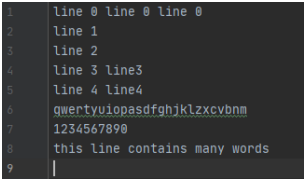
\includegraphics[width=0.6\linewidth]{photo/file_example}
	\caption{Исходный файл для тестов}
	\label{file_example}
\end{figure}

Тест с вводом символа l. Вывод в консоль на рис. \ref{test.1.console}, Результирующий
файл на рис. \ref{test.1.file}.

\begin{figure}[H]
	\centering
	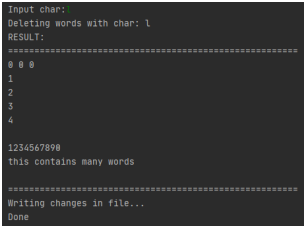
\includegraphics[width=0.6\linewidth]{photo/test.1.console}
	\caption{Тест №1 -- консоль}
	\label{test.1.console}
\end{figure}

\begin{figure}[H]
	\centering
	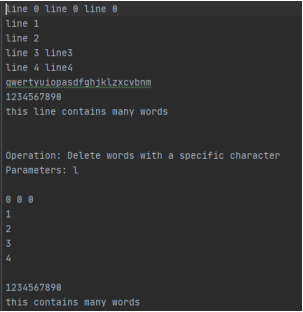
\includegraphics[width=0.6\linewidth]{photo/test.1.file}
	\caption{Тест №1 -- файл}
	\label{test.1.file}
\end{figure}

\newpage

Тест с вводом символа a. Вывод в консоль на рис. \ref{test.2.console}, Результирующий
файл на рис. \ref{test.2.file}.

\begin{figure}[H]
	\centering
	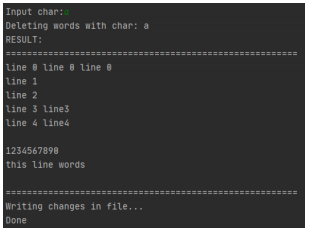
\includegraphics[width=0.6\linewidth]{photo/test.2.console}
	\caption{Тест №2 -- консоль}
	\label{test.2.console}
\end{figure}

\begin{figure}[H]
	\centering
	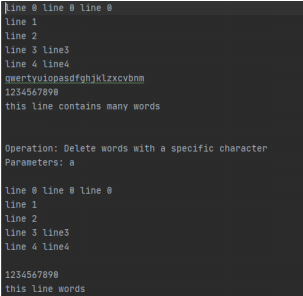
\includegraphics[width=0.6\linewidth]{photo/test.2.file}
	\caption{Тест №2 -- файл}
	\label{test.2.file}
\end{figure}

% test with character not included in text

Тест с вводом символа ','. 
Данного символа нет в тестовом файле,
поэтому содержимое текста не меняется.
Вывод в консоль на рис. \ref{test.3.console}, Результирующий
файл на рис. \ref{test.3.file}.

\begin{figure}[H]
	\centering
	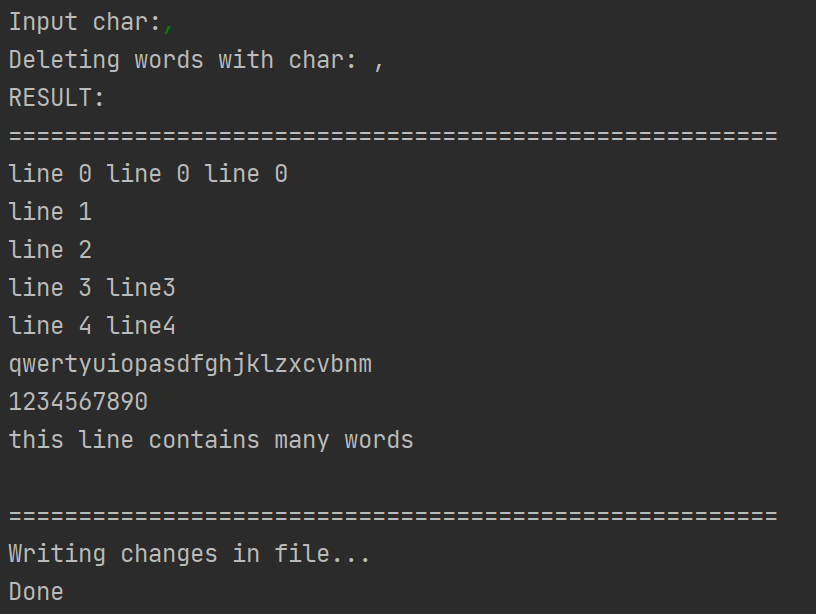
\includegraphics[width=0.6\linewidth]{photo/test.3.console}
	\caption{Тест №3 -- консоль}
	\label{test.3.console}
\end{figure}

\begin{figure}[H]
	\centering
	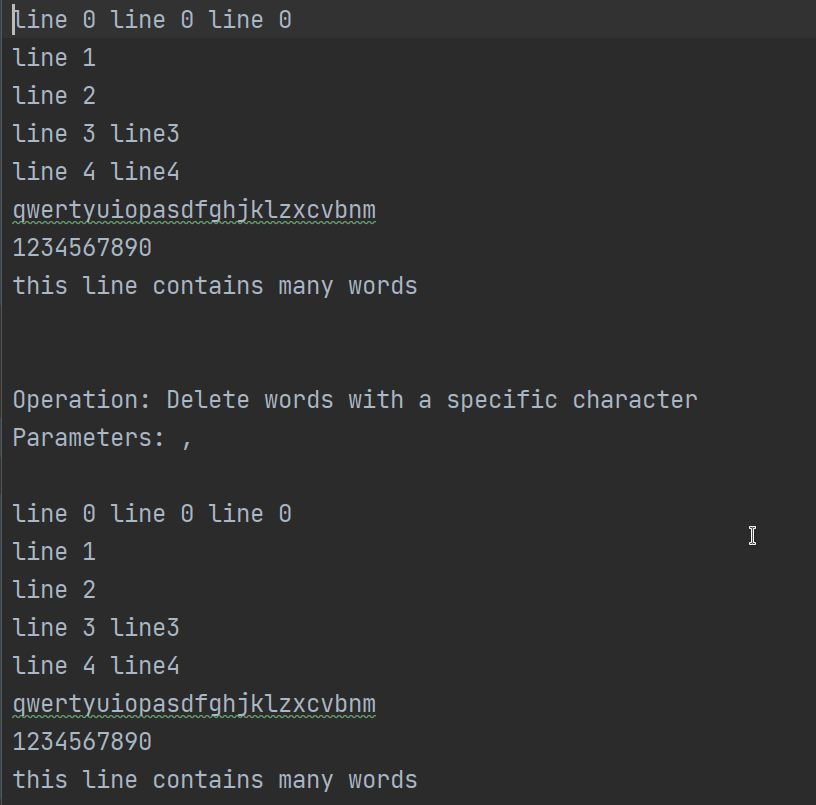
\includegraphics[width=0.6\linewidth]{photo/test.3.file}
	\caption{Тест №3 -- файл}
	\label{test.3.file}
\end{figure}